%%%%%%%%%%%%%%%%%%%%%%%%%%%%%%%%%%%%%%%%%%%%%%%%%%%%%%%%%%%%%%%%%%%%%%%%%%%%%%%%%%%%%%%%%%%%%%%%%%%%%%%%%%%%%%%%%%%%%%%%%%%%%%%%%%%%%%%%%%%%%%%%%%%%%%%%%%%
% This is just an example/guide for you to refer to when submitting manuscripts to Frontiers, it is not mandatory to use Frontiers .cls files nor frontiers.tex  %
% This will only generate the Manuscript, the final article will be typeset by Frontiers after acceptance.
%                                              %
%                                                                                                                                                         %
% When submitting your files, remember to upload this *tex file, the pdf generated with it, the *bib file (if bibliography is not within the *tex) and all the figures.
%%%%%%%%%%%%%%%%%%%%%%%%%%%%%%%%%%%%%%%%%%%%%%%%%%%%%%%%%%%%%%%%%%%%%%%%%%%%%%%%%%%%%%%%%%%%%%%%%%%%%%%%%%%%%%%%%%%%%%%%%%%%%%%%%%%%%%%%%%%%%%%%%%%%%%%%%%%

%%% Version 3.4 Generated 2018/06/15 %%%
%%% You will need to have the following packages installed: datetime, fmtcount, etoolbox, fcprefix, which are normally inlcuded in WinEdt. %%%
%%% In http://www.ctan.org/ you can find the packages and how to install them, if necessary. %%%

\documentclass[utf8]{frontiersSCNS}

%\setcitestyle{square} % for Physics and Applied Mathematics and Statistics articles
\usepackage{url,hyperref,lineno,microtype,subcaption}
\usepackage[onehalfspacing]{setspace}

\linenumbers


% BELOW TAKEN FROM rticles plos template
%
% amsmath package, useful for mathematical formulas
\usepackage{amsmath}
% amssymb package, useful for mathematical symbols
\usepackage{amssymb}

% hyperref package, useful for hyperlinks
\usepackage{hyperref}

% graphicx package, useful for including eps and pdf graphics
% include graphics with the command \includegraphics
\usepackage{graphicx}

% Sweave(-like)
\usepackage{fancyvrb}
\DefineVerbatimEnvironment{Sinput}{Verbatim}{fontshape=sl}
\DefineVerbatimEnvironment{Soutput}{Verbatim}{}
\DefineVerbatimEnvironment{Scode}{Verbatim}{fontshape=sl}
\newenvironment{Schunk}{}{}
\DefineVerbatimEnvironment{Code}{Verbatim}{}
\DefineVerbatimEnvironment{CodeInput}{Verbatim}{fontshape=sl}
\DefineVerbatimEnvironment{CodeOutput}{Verbatim}{}
\newenvironment{CodeChunk}{}{}

% cite package, to clean up citations in the main text. Do not remove.
\usepackage{cite}

\usepackage{color}

% Below is from frontiers
%
\bibliographystyle{frontiersinSCNS}
% Use doublespacing - comment out for single spacing
%\usepackage{setspace}
%\doublespacing


% Leave a blank line between paragraphs instead of using \\


\def\keyFont{\fontsize{8}{11}\helveticabold }


%% ** EDIT HERE **
%% PLEASE INCLUDE ALL MACROS BELOW

%% END MACROS SECTION


% tightlist command for lists without linebreak
\providecommand{\tightlist}{%
  \setlength{\itemsep}{0pt}\setlength{\parskip}{0pt}}




\def\Authors{
  Francisco Cervantes\,\textsuperscript{1,2*},
  Res Altwegg\,\textsuperscript{1},
  Francis Strobbe\,\textsuperscript{2},
  Andrew Skowno\,\textsuperscript{3},
  Vernon Visser\,\textsuperscript{1},
  Michael Brooks\,\textsuperscript{4},
  Yvan Stojanov\,\textsuperscript{2},
  Douglas M. Harebottle\,\textsuperscript{5},
  Nancy Job\,\textsuperscript{3}}

\def\Address{

  \textsuperscript{1} Centre for Statistics in Ecology, the Environment
and Conservation, University of Cape Town,  Cape Town,   South Africa
  
  \textsuperscript{2} Operational Directorate Natural Environment, Royal
Belgian Institute of Natural Sciences,  Brussels,   Belgium
  
  \textsuperscript{3} South African National Biodiversity
Institute, Kirstenbosch Research Centre,  Cape Town,   South Africa
  
  \textsuperscript{4} FitzPatrick Institute of African
Ornithology, University of Cape Town,  Cape Town,   South Africa
  
  \textsuperscript{5} Risk and Vulnerability Science Centre, Sol Plaatje
University,  Kimberley,   South Africa
  }

  \def\corrAuthor{Francisco Cervantes}\def\corrAddress{University of
Cape Town\\Rondebosch\\Cape Town, State XX, 7700 South
Africa}\def\corrEmail{\href{mailto:f.cervantesperalta@gmail.com}{\nolinkurl{f.cervantesperalta@gmail.com}}}
  \def\firstAuthorLast{Cervantes {et~al.}}
  
  
  
  
  
  
  
  
  
  
  
  
  
  
  
  


\begin{document}

\onecolumn
\firstpage{1}


\title[BIRDIE biodiversity data pipeline]{BIRDIE: A data pipeline to
inform wetland and waterbird conservation at multiple scales}
\author[\firstAuthorLast]{\Authors}
\address{} %This field will be automatically populated
\correspondance{} %This field will be automatically populated

\extraAuth{}% If there are more than 1 corresponding author, comment this line and uncomment the next one.
%\extraAuth{corresponding Author2 \\ Laboratory X2, Institute X2, Department X2, Organization X2, Street X2, City X2 , State XX2 (only USA, Canada and Australia), Zip Code2, X2 Country X2, email2@uni2.edu}


\maketitle

\begin{abstract}

Efforts to collect ecological data have intensified over the last decade. This is especially true for freshwater habitats, which are among the most impacted by human activity and yet lagging behind in terms of data availability. Now, to support conservation programmes and management decisions, these data need to be analysed and interpreted; a process that can be complex and time consuming. The South African Biodiversity Data Pipeline for Wetlands and Waterbirds (BIRDIE) aims to help fast and efficient information uptake, bridging the gap between raw ecological datasets and the information final users need. BIRDIE is a full data pipeline that takes up raw data, and estimates indicators related to abundance, distribution and diversity of waterbirds, while keeping track of their associated uncertainty. At present, most functionality focuses on the assessment of waterbird populations in South Africa using two citizen-science bird monitoring datasets, namely: the African Bird Atlas Project and the Coordinated Waterbird Counts. In addition, a suite of environmental layers help contextualise waterbird population indicators, and link these to the ecological condition of the supporting wetlands. In the future,  we aim to develop more indicators specific to the ecological structure and function of wetlands. Data processing is conveniently organised in modules that can be run independently, and include tasks, such as: data cleaning, statistical analysis, and computation of indicators at multiple temporal and spatial scales. Both data and indicators are accessible to end users through an online portal and web services. Envisioned users of BIRDIE include government officials, conservation managers, researchers and the general public, all of whom have been engaged throughout the project. Acknowledging that conservation programmes run at multiple spatial and temporal scales, we have developed a granular framework in which waterbird population indicators are estimated at small scales, and then these are aggregated to compute similar indicators at broader scales. The online portal is designed to provide spatial and temporal visualisation of the indicators using maps, time series and pre-compiled reports for species, sites and conservation programmes. This paper describes the structure of the BIRDIE pipeline and the technical features underpinning its components.

%All article types: you may provide up to 8 keywords; at least 5 are mandatory.
\tiny
 \keyFont{ \section{Keywords:} Biodiversity informatics, Citizen science, Data pipeline, Waterbirds, Wetlands, Species distribution, Species Abundance, Diversity } 

\end{abstract}

\hypertarget{introduction}{%
\section*{Introduction}\label{introduction}}
\addcontentsline{toc}{section}{Introduction}

Freshwater ecosystems are among the most productive, biodiverse, and
efficient at capturing and storing carbon (Convention on Wetlands,
2021). Unfortunately, they are also among the most impacted by human
activity (Convention on Wetlands, 2021; Skowno et al., 2019), and
climate change will likely exacerbate the pressure on freshwater
resources. This is particularly true for the African continent, home to
some of the largest wetlands, which not only host a wealth of freshwater
species, but are also key in supporting human communities (Stephenson et
al., 2020). Such critical issues have fuelled unprecedented efforts to
collect and mobilise freshwater biodiversity data (Dallas et al., 2021;
Wetzel et al., 2015).

While we must strive to keep monitoring programmes that deliver data
funded and alive, it is clear that data on their own are not enough
(MacFadyen et al., 2022). If we are to take effective action to stop
ecosystem degradation, it is important that data are analysed to extract
indicators that are meaningful for decision- and policy-making
(Harebottle and Underhill 2016, Jetz et al., 2019; Stephenson et al.,
2017). Furthermore, with continuous data collection, we need to
implement workflows that update indicators and support decisions in a
timely fashion (MacFadyen et al., 2022; Yenni et al., 2019). Automated
data pipelines allow us to keep datasets updated and free of errors
(Yenni et al., 2019), make model-based forecasts, and evaluate previous
forecasts in light of new data (White et al., 2019). These modern and
automated data workflows require multidisciplinary skills in ecology,
statistics, data science, and software development, but their end
products should ideally be free, accessible and easy to interpret
(Stephenson et al., 2017). It would also be desirable that they
integrate multiple datasets and environmental layers to produce a
holistic understanding of biodiversity structure and function (MacFadyen
et al., 2022).

South Africa is leading the African continent in terms of biodiversity
data availability (Barnard et al., 2017), with successful
citizen-science programmes such as the Southern African Bird Atlas
Project (Brooks et al., 2022), and biodiversity data platforms, such as
the Biodiversity Advisor (SANBI, 2023) or the Freshwater Biodiversity
Information System (FBIS, Dallas et al., 2021). In contrast, dashboards
and tools that facilitate the timely uptake of information and unlock
the utility of current data are still limited. There is also an
imbalance in data availability across taxonomic groups and habitats.
Regular monitoring of the status, distribution and condition of wetlands
ecosystems is urgently required to understand environmental pressures on
wetland habitats, but challenges associated with limited human and
budget capacity hamper the collection of the necessary data. Conversely,
available waterbird species data are rich in detail and coverage, and
could provide a stronger basis for both adaptive management and
reporting at priority wetland sites.

Here, we describe a data pipeline that implements a workflow of wetland-
and waterbird-related biodiversity data, the South African Biodiversity
Data Pipeline for Wetlands and Waterbirds (BIRDIE). At present, most of
BIRDIE's functionality focuses on computing indicators related to
waterbird distribution and abundance, which are considered the minimum
set of variables necessary to study changes in species populations
(Pereira et al.~2013, Jetz et al.~2020). BIRDIE utilises two long-term
citizen-science programmes that have collected waterbird data in South
Africa for more than two decades, and are still active: the Southern
African Bird Atlas Project (SABAP; Brooks et al., 2022) and the
Coordinated Waterbird Counts (CWAC; FIAO, 2022). Apart from waterbird
data, BIRDIE uses and serves ancillary environmental data for
contextualising the aforementioned waterbird population variables, and
also for describing the state of the wetlands that support them. In a
next phase, we plan to expand the functionality of the pipeline to
provide indicators of wetland ecosystem structure and function.

BIRDIE is embedded into the South African National Biodiversity
Institute (SANBI) biodiversity informatics infrastructure and it was
conceived as a tool to inform environmental strategies, identify
priorities for the protection and sustainable use of biodiversity, and
to guide land-use management. Because such policy-linked objectives
require updated and timely information, the pipeline was designed to run
periodically (yearly in principle), and automatically (but supervised).
Currently, BIRDIE provides indicators for South Africa only, but in the
future we expect to expand its coverage to other African countries. In
what follows we describe BIRDIE's data pipeline workflow from data
acquisition to display of final outputs, as well as the technologies we
have used and the general modelling frameworks adopted.

\hypertarget{framework-and-target-users}{%
\section*{Framework and target users}\label{framework-and-target-users}}
\addcontentsline{toc}{section}{Framework and target users}

Indicators on the state of biodiversity have been adopted by a range of
multilateral environmental agreements including the United Nations
Convention on Biological Diversity (CBD, 2022) and Sustainable
Development Goals (SDGs; UN, 2022). New indicators are under development
and established processes, such as the International Union for the
Conservation of Nature (IUCN, 2022) species red-listing efforts, are
receiving renewed attention (Han et al., 2017). With these indicators
come various global and national initiatives and targets for reducing
rates of biodiversity loss (Mace et al., 2018). Essential Biodiversity
Variables (EBVs) have been conceptualised and developed to help
standardise and improve interoperability of biodiversity data for
monitoring (Pereira et al., 2013).

Within this framework, BIRDIE gives support to both national and
international programs contributing information about the state of
waterbird populations in South Africa, with a view to expand to the
Southern Africa region. We focus primarily on species population EBVs,
with the assessment of waterbird abundance, distribution and diversity,
and changes of these over time (Jetz et al., 2019; Kissling et al.,
2018). Species diversity falls under the community composition EBVs
rather than species populations.

At the international scale, South Africa is signatory to the Ramsar
Convention (Convention on Wetlands, 2021), hosts 28 Wetlands of
International Importance, and needs to produce reports on the state of
sites every three years. Change in condition and extent of wetland
habitat, as well as those Ramsar Criteria invoked when listing the
different sites as internationally important are all core reporting
requirements. These include changes in overall abundance and
distribution of waterbirds at these sites, with special attention to
threatened and migratory species.

National reports must also be compiled for the Agreement on the
Conservation of African-Eurasian Migratory Waterbirds (AEWA; UNEP,
2022), another international agreement, framed under the Convention on
Migratory Species, and focused on protecting migratory waterbirds and
their habitats. Reporting for this agreement requires the full suite of
EBVs outlined earlier in this section, now specific to migratory
species, namely, abundance, distribution, diversity, and changes in
these over time. Within South Africa, there is alignment and cooperation
between Ramsar and AEWA, and as such, reporting on the change in wetland
extent and condition is also relevant.

At the national level, South Africa produces a National Biodiversity
Assessment every four years, which constitutes the main reporting tool
of the state of biodiversity in the country, and informs policy and
conservation strategies (Skowno et al., 2019). At the same time, there
are regular efforts to address the conservation status of South African
species within the IUCN Red-List framework. Changes in abundance and
distribution of species are key in these assessments to track and report
on population trends, and shifts in species ranges and community
diversity.

Keeping these main reporting channels in mind, BIRDIE also intends to
support local management actions and basic research. Site-scale wetland
monitoring is severely limited in South Africa, lagging far behind
monitoring of other aquatic ecosystems such as rivers and estuaries.
Managers ideally need to report on the state of the wetland (e.g.,
wetland condition, flux in surface water extent) as well as the species
that the wetland supports, including species of special concern. Local
waterbird and wetland information can facilitate the development of
site-specific management actions and management plans, and support
permitting decisions. At the same time, linking the local manager inputs
and feedback into the data pipeline closes the gap between large-scale
assessments and local data collection. The data pipeline also allows
citizen scientists to more actively interact with the data they have
collected, and to see it taken up into the statistical analyses and data
visualisations.

\hypertarget{input-data}{%
\section*{Input data}\label{input-data}}
\addcontentsline{toc}{section}{Input data}

South Africa needs to monitor its biodiversity to inform decisions that
affect the environment, and to fulfil reporting obligations linked to
international conventions. Fortunately, we have a number of long-running
citizen science projects that help monitor waterbird populations
throughout the country. At its core, the project leverages two
bird-related datasets: the Coordinated Waterbird Counts (CWAC) and the
South African Bird Atlas Project (SABAP2), which is part of the larger
African Bird Atlas Project (ABAP). These datasets have well established
citizen scientist support and offer information about: 1) bird
abundance, with waterbird counts taken twice a year at 731 water bodies
across Southern Africa (mostly South Africa) since 1992, and 2) species
occurrence, with visits to a grid of pentads (5' x 5' grid cells)
initiated in 2007 and covering several African countries.

The Coordinated Waterbird Counts project provides regular counts of all
waterbirds at just over 700 sites throughout South Africa. The project
was launched in 1992 and since then, it has accumulated a long time
series for many sites. However, not all sites have been monitored since
the start of the project, some regions are better represented than
others, and not all sites have been monitored continuously (Figure 3).
Waterbird species have diverse habitat requirements and life histories;
some use the same sites year-round, whereas others are migratory. To
capture this diversity, CWAC counts are carried out twice per year: one
in mid-summer and one in mid-winter. These data are noisy because it is
difficult to count waterbirds precisely, but with appropriate
statistical analyses, they can reveal long-term temporal trends and
seasonal fluctuations in waterbird populations. Waterbird population
sizes and trends are important reporting parameters for international
agreements such as the Ramsar Convention, or AEWA.

ABAP offers occurrence, rather than abundance data. In ABAP, volunteers
collect checklists of all birds observed over a grid of pentads (5' x 5'
minute grid) covering different African countries. We are currently
restricting our analysis to South Africa, and therefore we are using the
SABAP2 component of ABAP (Figure 4). However, in the future we would
like to expand our functionality to cover other countries contributing
data to ABAP, such as Kenya or Nigeria. Under the SABAP2 protocol, which
started in 2007, observers need to spend at least two hours of intensive
birding at a pentad and are asked to visit as many habitats within it as
possible. They can add new species for up to five days. SABAP2 currently
has ca. 17 million records, and \textgreater{} 2 million records are
added per year. The structured sampling protocol, together with the
spatial and temporal extent of SABAP2 allow us to examine how bird
distributions are changing over time, although statistical modelling is
required to account for imperfect detection and sampling biases (Figure
4).

There are a variety of other data sources that BIRDIE uses for adding
environmental information into its analytical workflows. Most of these
data sources are conveniently accessed through Google Earth Engine, such
as TerraClimate (Abatzoglou et al., 2018), the JRC surface water dataset
(Pekel et al., 2016), MODIS Vegetation Indices (Didan, Kamel, 2015) and
Digital Elevation Models (DEM, (Yamazaki et al., 2017). Other data not
yet available on Google Earth Engine, such as the National Wetland Map
(SANBI, in prep.) are managed independently.

\hypertarget{indicators-and-statistical-methods}{%
\section*{Indicators and statistical
methods}\label{indicators-and-statistical-methods}}
\addcontentsline{toc}{section}{Indicators and statistical methods}

Capturing good quality raw data is a fundamental first step to monitor
the state of biodiversity. However, raw data reflect not only the
biological signal of interest but also the sampling process, which is
typically spatially biased and subject to imperfect detection (Yoccoz et
al., 2001). Therefore, some level of statistical analysis is required to
estimate the state of the system of interest, and separate it from
observational artefacts introduced by the observation process used for
capturing the data (Gimenez et al., 2014; King, 2014; Yoccoz et al.,
2001). The BIRDIE pipeline broadly uses two types of models: 1)
occupancy models (Altwegg and Nichols, 2019; MacKenzie et al., 2002) to
estimate the probability of a species being present at the different
SABAP2 pentads, and 2) state-space models (Buckland et al., 2004; Newman
et al., 2014) to estimate the number of individuals at the sites
monitored by the CWAC programme. Contrary to raw observations (counts
and detection/non-detection of a species), model-based estimates
(abundance and occupancy probabilities) allow us to quantify
uncertainty.

The variety of end-user needs requires a pipeline that provides
waterbird population indicators at multiple spatial and temporal scales.
Therefore, in addition to estimating basic occupancy and abundance at
small scales (i.e., individual site/pentad), the BIRDIE pipeline
produces other high-level indicators obtained by aggregation (Table 1).
The idea is to follow a process whereby raw data are used to inform
models that estimate indicators at the smallest temporal and spatial
scales possible, and then to aggregate these estimates at larger scales,
as required. For example, species abundance can be estimated for a set
of regularly monitored wetlands in South Africa, and these site-specific
estimates can then be combined to calculate an abundance index for all
sites as a group. We can follow this procedure to estimate abundance and
occupancy probabilities at national, regional and local levels, as well
as for specific groups of wetlands (e.g., designated Ramsar sites,
estuaries or artificial sites).

The main indicators computed by the BIRDIE pipeline for waterbird
species are:

\begin{itemize}
\item
  Abundance: estimated for CWAC sites in two seasons per year. For each
  species, only those wetlands with at least a ten-year coverage between
  1997 and 2021 are analysed statistically.
\item
  Occurrence: estimated for ABAP pentads on an annual basis.
\item
  Diversity: the simplest and most easily understood metric is species
  richness. Species richness can be calculated based on the occupancy
  analysis, by summing occupancy probabilities of all species
  potentially present in each pentad, to estimate the expected number of
  species present.
\item
  Important records: sightings of rarities, invasive species. Although
  this information does not require any statistical processing, it does
  make particular records more visible.
\end{itemize}

In addition to estimates of static indicators, the pipeline also
estimates their associated dynamics, such as: changes in abundance,
occupancy probabilities and diversity. The temporal reference for these
dynamics can also vary ranging from a single season to multiple years
(typically ca. 5 years, for short-term changes, and ca. 15 years for
long-term changes).

It is important that uncertainty is correctly propagated when
aggregating, and also when estimating dynamic indicators. We work in a
Bayesian framework and use the posterior distribution of occupancy
probabilities and species abundance to define indicators at the various
scales. Working with full posterior distributions allows us to
conveniently keep track of the uncertainty in the estimates used as
building blocks for other derived indicators.

\hypertarget{delineating-species-distributions}{%
\subsection*{Delineating species
distributions}\label{delineating-species-distributions}}
\addcontentsline{toc}{subsection}{Delineating species distributions}

Occupancy models are fitted to detection/non-detection data from SABAP2
to delineate the distribution of waterbird species and its dynamics over
time. Within the SABAP2 framework, observers visit pentads and make a
list of the bird species detected during the visit. We assume that
observers identify species correctly and only list species observed (the
rigorous vetting process of SABAP2 data justifies this assumption), but
non-detections may be caused by either species not being present in the
pentad or by observers not being able to detect them, when present.
Therefore, occupancy models describe two processes simultaneously: i)
the underlying occupancy of the sites (pentads), and ii) the observation
process whereby species present might or might not be observed.

More precisely, we define \(z_{jt}\) to be the true occupancy of site
\(j\) in year \(t\), which can be 1 (if species present) or 0 (if
species absent) and has distribution:

\[z_{jt}|\psi_{jt} \sim \textrm{Bernoulli}(\psi_{jt})\]

where \(\psi_{jt}\) is the occupancy probability at site \(j\) and year
\(t\). The logit transformation of \(\psi_{jt}\) can be modelled as a
linear combination of covariates and smooth functions of covariates,
such that:

\[\textrm{logit}(\psi_{jt}) = \boldsymbol{x}_{jt}^\intercal \boldsymbol{\beta} + \sum_{k=1}^K f_k(u_{jk})\]

where \(u_{jk}\) is a smooth function of the covariate \(u_k\), which is
defined as

\[f_k(u_{jk}) = \sum_{l=1}^L \textrm{B}_l(u_{jkl})\gamma_{jkl}\]

where the smooth function \(f\) is represented by a set of \(L\) basis
functions \(\textrm{B}_l\) evaluated at the value of the covariates
associated with site \(j\) at year \(t\)

We can then write the likelihood of observation as:

\[y_{ij}|z_{jt},p_{ij} \sim \textrm{Bernoulli}(z_{jt}p_{ij})\]

The probability of detection of a species that is present in site \(j\)
on visit \(i\) is denoted by \(p_{ij}\). Following the same logic as for
the probability of occupancy, the logit transformation of \(p\) is
modelled as a linear combination of covariates and smooth functions:

\[\textrm{logit}(p_{ij})= \boldsymbol{w}_{ij}^\intercal \boldsymbol{\alpha} + \sum_{h=1}^H f_h(v_{ih})\],

Spatial, spatio-temporal, and unstructured random effects can be
specified for either occupancy or detection probabilities to account for
variation across sites, observers and visits, not accounted for by the
covariates incorporated in the models.

Each checklist is treated as an independent survey, but occupancy is
assessed on a yearly basis. This means that if a species is detected in
any one survey it is considered present that year. Therefore, missing a
species because it left the site is considered part of the observation
process and not the occupancy process. Migratory birds, for example, are
considered present at a site even if they are only there for part of the
year.

We are fitting single-season occupancy models without spatial random
effects to most species. However, all models incorporate random effects
to account for pentad- and observer-specific detection probabilities. If
model diagnostics indicate poor model fit (see model diagnostics section
below), we try incorporating spatial random effects for occupancy
probabilities with an exponential decay function. Currently, we fit the
models in R (R Core Team, 2022), in a Bayesian framework using the
package spOccupancy (Doser et al., 2022), and running three MCMC chains
for 20,000 iterations, with a thinning interval of 20. We use
non-informative priors for all parameters when no information from other
years is available, but we incorporate information obtained from other
model fits if available, by centering the priors on the closest model's
posterior means. However, it is important noticing that modelling
details may differ among species and may be updated in the future.

\hypertarget{estimating-abundance-and-population-trends}{%
\subsection*{Estimating abundance and population
trends}\label{estimating-abundance-and-population-trends}}
\addcontentsline{toc}{subsection}{Estimating abundance and population
trends}

State-space models (Buckland et al., 2004; Newman et al., 2014) are used
to describe and understand dynamic systems that may not be perfectly
observed . Within this framework, we consider waterbird abundance to be
a process that evolves over time, and which we observe during visits to
CWAC sites. However, counts conducted by observers are distorted by
imperfect detection that translates into counting errors. By counting
repeatedly over time, and assuming that abundance evolves smoothly over
time compared to observation error, we can disentangle these two
processes.

We consider that the observed counts (\(y_i\)) at sampling occasion
\(i\) (generally there were two sampling occasions per year, one in
mid-summer and one in mid-winter), at any given site, arise from a
Poisson(\(\lambda_i\)) distribution

\[y_i \sim \textrm{Poisson}(\lambda_i)\]

And we model the log of the intensity \(\lambda_i\) as:

\[\log{(\lambda_i)} \sim N(\mu_i, \sigma^2)\]

where \(\mu_i\)is the mean abundance of waterbirds present at a site on
sampling occasion \(i\) and \(\sigma^2\) is the corresponding variance
of the observers counting error, both in the log scale. Therefore,
counts depend both on the number of waterbirds present on site, and on
errors in the counts of these birds.

To model changes in waterbird abundance between the two-seasons of year
\(t\), we define \(s_t\) to be the summer abundance and \(w_t\) the
winter abundance. Note that there might be multiple counts in a single
year and season, but the underlying true abundance is considered to stay
constant in any given year and season (for clarity, note also that while
sampling occasions were indexed by \(i\), years are indexed by \(t\)).
Thus, the expected (log) abundance for any given count can be written as

\[\mu_{i} = s_t \textrm{summer} + w_t \textrm{winter}\]

where `summer' is an indicator variable that takes on the value 1 in
summer and 0 in winter, and `winter' is the opposite. We then define
abundance dynamics as:

\[s_t = s_{t-1} + \beta_t\] \[w_t = s_t + \xi_t\]

where \(\beta_t\) corresponds to the change in summer abundance from
year \(t-1\) to year \(t\), and \(\xi_t\) is the difference between
summer and winter abundance, both in the log scale. If exponentiated,
these parameters can be interpreted as the rate of change in the
population and the winter-to-summer ratio of the population,
respectively.

We impose relatively smooth changes in abundance by defining
autocorrelation in \(\beta_t\) and \(\xi_t\) terms over time. In
addition, we define relationships between the rate of change in the
population \(\beta_t\) and environmental covariates. These relationships
facilitate the estimation of abundance for those years in which counts
are missing, and it is particularly useful to contain uncertainty in
long periods with missing data between counts. Thus, we set

\[\beta_{t} = \phi\beta_{t-1} + \eta_{t-1} + \zeta_{t-1}\]
\[\xi_{t} = \xi_{t-1} + \epsilon_{t-1}\]

where \(\phi\) lies between zero and one, and it defines an
autoregressive term on \(\beta_{t-1}\); \(\eta_t\) captures the effect
of covariates in the expected change in abundance, and can be expanded
to \(\gamma^{\intercal}\mathrm{U}\), where \(\mathrm{U}\) is a matrix of
covariate values and \(\gamma\) a vector of coefficients; \(\zeta_t\)
and \(\epsilon_t\) are random variables that represent change in
abundance change, and change in winter to summer ratio, respectively.

We mentioned at the beginning that this model applies to each monitored
site. However, we have multiple sites, and counts are often missing for
some seasons or even full years. To facilitate the estimation of
abundance with missing data, we borrow information from sites with
counts, by defining a hierarchical structure such that:

\[\zeta_{tj} \sim N(0, \sigma^2_{\zeta t})\]
\[\epsilon_{tj} \sim N(0, \sigma^2_{\epsilon t})\]

so that random changes at any site and year come from a common
distribution of changes across all sites for that year. These
distributions are normal with variances \(\sigma^2_{\zeta t}\) and
\(\sigma^2_{\epsilon t}\) for changes in abundance and winter to summer
ratio, respectively.

We fit these models in R (R Core Team, 2022) with the additional
functionality provided by JAGS (Plummer, 2003) using the package jagsUI
(Kellner, 2021). We work on a Bayesian framework, using non-informative
priors, and running three chains for 10,000 iterations each. Similar to
the occupancy models, these are the details of the models we are working
with at the moment, and they are intended to give an idea of the type of
model we are using. These models might be updated in the future and the
updated modelling details will be published on the BIRDIE website.

\hypertarget{data-and-model-diagnostics}{%
\subsection*{Data and model
diagnostics}\label{data-and-model-diagnostics}}
\addcontentsline{toc}{subsection}{Data and model diagnostics}

The pipeline needs to run for a multitude of species, with different
ecological requirements and geographical distributions. Therefore,
finding a model that suits all species is challenging. Not only may a
model not be a good fit for a particular species, but the algorithms
used for fitting the model may fail to converge due to characteristics
of the data.

In a first control stage, we have defined the minimum requirements that
the data should meet to enter the model-fitting process. Species that
have been observed in five or less pentads in a year are considered to
not have enough data to inform an occupancy model. Similarly, we chose
only those CWAC sites that have been counted at least ten times between
1993 and 2021, to fit state-space models. Otherwise, data tend to be too
sparse to assess trends in abundance reliably. These thresholds are
based on our own experiences working with these data, and they are
considered to be the minimum requirements for models to converge
successfully. However, meeting these requirements does not guarantee
model convergence or a good fit. To keep track of potential issues
arising during model fitting, and to improve the algorithms of the
pipeline, each time the pipeline runs it generates several reports that
are later examined.

To decide whether any occupancy or state-space model converges, we
calculate the Gelman-Rubin (Rhat) diagnostic (Gelman et al., 2014) for
each estimated parameter. These diagnostics are then tabulated and
stored for future revision. Any Rhat value above 1.1 or below 0.9 is
considered to represent lack of convergence. Distinctive characteristics
of the models with convergence issues are explored and addressed on a
case by case basis, after the pipeline has finished running.

In addition to convergence, we assess goodness of fit using posterior
predictive checks (Doser et al., 2022; Gelman et al., 2014). This
procedure compares some quantity of interest calculated using
pseudo-data simulated from the model posterior distribution, with that
same quantity calculated from the observed data. In a well-fitting model
we would expect real and synthetic data to produce similar values. For
occupancy models, we produce simulated detection/non-detection data for
each site, species and year and compute the expected number of
detections out of as many visits as there were in the data. We compare
the results of the simulations with the observed number of detections
recorded in the data using Chi-square tests (Doser et al., 2022). For
state-space models we follow a similar procedure, but instead of
simulating detection/non-detection data for one year, we simulate count
data for summer and winter, and aggregate these in a single annual
count. Results from the goodness of fit Chi-square tests are also
tabulated and stored for revision. Significant deviations detected with
these tests are addressed for each case individually.

Due to the computational burden of the pipeline, it is not possible to
run multiple models for each species, site and year, to perform model
selection. Therefore, model selection is performed on a sample of
species, selected to have representation of common and scarce taxa, but
that are otherwise selected arbitrarily. Our general approach has been
to include a rich set of variables that we believe can explain the main
environmental gradients within our geographical range, without paying
too much attention to multi-collinearity and overfitting. We are
therefore cautious about making causal inference or predictions outside
of the range of the data, and so should be other users.

\hypertarget{systems-and-technology}{%
\section*{Systems and technology}\label{systems-and-technology}}
\addcontentsline{toc}{section}{Systems and technology}

In this section we describe the technology that underpins the flow of
data along the pipeline until it is transformed into indicators that are
presented to the BIRDIE user. BIRDIE's data, code and outputs are stored
and run on three main systems (Figure 5): the Africa Bird Data servers,
and the two BIRDIE servers (servers A and B).

The Africa Bird Data servers are hosted at the FitzPatrick Institute for
African Ornithology, University of Cape Town, and contain the CWAC and
ABAP databases. They also serve these data through an Application
Programming Interface (API).

BIRDIE's server A is the access point of the final user to the
information generated by the pipeline. This information is stored in a
data mart, which in essence, is a MySQL database (version 8.0.27), a
widely used, open source, relational database management system. Its
main objective is to store the outputs of BIRDIE's data analyses and
provide easy and flexible access to the final user. At the same time,
the structure of the database ensures that inputs and outputs conform to
a given standard, and creates security back-ups for the stored data. The
main mechanism BIRDIE uses to present data to the user is through
OpenAPI web services (OpenAPI Specification, Version 3.1.0), which was
designed to provide a standard interface for documenting and exposing
APIs. The public web services offered by the OpenAPI give users the
flexibility to access and download data from the database without being
constrained by the specific functionality of a web application. This
technology facilitates the integration of BIRDIE's outputs into other
workflows. However, for the user that is interested in readily accessing
the information through a dashboard, we have deployed a web application,
written in HTML5, CSS, and the most common and popular JavaScript
libraries, including OpenLayers (\url{https://openlayers.org/}) and
Plotly (\url{https://plotly.com/}). Among other elements (see section
6), the web application features a map viewer, based on mviewer
(\url{https://mviewer.netlify.app/en/}), a free and open-source
cartographic application, that has an easy-to-use and intuitive
interface.

If we thought of server A as being the face of the pipeline, server B
would be the brain. All the functionality in this server revolves around
statistical modelling. This server connects with the Africa Bird Data
servers to obtain CWAC and ABAP data, and with other external systems,
such as Google Earth Engine or SANBI servers to obtain environmental
information. It then runs the main analytical modules of the pipeline,
where occupancy and state-space models are fitted. At the time of
writing, the analytical workflows were supported by an Intel Xeon Dual 8
core, with 64 GB RAM and an 8 TB hard drive. The model outputs are made
available to server A, where they are incorporated into the data mart,
used to compute derived high-level indicators by aggregation (see
section 4), and prepared to be presented to the final users.

In terms of code structure, the BIRDIE data pipeline consists of several
fundamental building blocks or modules. The first module, which we call
the data source layer (Figure 5) hosts and curates the raw data. The
second module, the analysis layer, analyses the data and estimates the
fundamental quantities of interest, like abundance and occurrence of
each species at each wetland or pentad. The third module consists of the
data mart where the outputs of the analyses are stored and indicators
are aggregated or disaggregated to multiple scales. The final module
serves the information to the user via APIs, web services and a web
application. The modular structure of BIRDIE enables us to maintain and
update individual parts independently. For example, we could replace the
current statistical routines with more efficient ones without changing
the other parts of the pipeline. Or we could add new indicators to the
data mart layer without needing to change the statistical routines that
produce the underlying components.

\hypertarget{web-application}{%
\section*{Web application}\label{web-application}}
\addcontentsline{toc}{section}{Web application}

To cater for different user needs, BIRDIE's web application offers four
main menus that provide access to the pipeline outputs in different ways
(see Figure 6):

\begin{enumerate}
\def\labelenumi{\arabic{enumi}.}
\item
  An exploration map. Through this menu the user can explore the
  different indicators BIRDIE computes on a map. This spatial framework
  can be configured to display information layers, such as occupancy
  probabilities for ABAP pentads or waterbird abundance at CWAC sites.
  Users can also zoom in and out to find the scale that best fits their
  needs. In addition to this, there are also environmental layers that
  can be overlaid to provide context and generate hypotheses on what
  might be driving the observed indicators.
\item
  Site and species summaries, are detailed reports elaborated for users
  focused on some sites or species in particular, rather than in general
  exploration. At the moment, site summaries are only available for
  those sites that have sufficient CWAC data to be included in BIRDIE's
  data analysis step. These reports contain a description of the
  site/species, links to other resources of interest (e.g., to criteria
  motivating declaration of Ramsar site or IUCN conservation status) and
  summaries prepared from BIRDIE's indicators. These reports can be
  exported as a document, and BIRDIE's data used for generating the
  reports can be accessed through the data mart and downloaded in common
  formats such as .json or .csv.
\item
  Reporting tools. We mentioned in section 2 that BIRDIE was developed
  to support reports for national and international conservation
  programmes. In this menu, users interested in elaborating, or
  accessing the information underpinning these reports, will find this
  information conveniently packed in programme-specific summaries.
  Similar to site and species summaries, reports for conservation
  programmes can also be printed, and the data used to compute
  statistics and create plots can be downloaded.
\item
  Web services. Through this menu users can access BIRDIE's API and
  retrieve its outputs in the most flexible way. It is through BIRDIE's
  API that all maps and plots in the web application are produced. By
  accessing this functionality directly, users can download the data
  themselves and incorporate them into their own workflows.
\end{enumerate}

\hypertarget{discussion}{%
\section*{Discussion}\label{discussion}}
\addcontentsline{toc}{section}{Discussion}

Data on biodiversity and related environmental drivers are collected at
increasingly faster rates. Although these data can be accessed to
support decisions at various levels, it can be difficult for decision
makers to extract relevant information in a timely fashion (MacFadyen et
al., 2022; Stephenson et al., 2017). Apart from data availability and
accessibility, obstacles for using biodiversity data in decision-making
include (MacFadyen et al., 2022; Stephenson et al., 2017): lack of
analysis and interpretation, lack of technical accessibility with
excessive use of jargon, and timely use of data. Here, we introduce
BIRDIE, the South African Biodiversity Data Pipeline for Wetlands and
Waterbirds; a data pipeline that aims to provide the information needed
for making evidence-based decisions on wetlands and waterbirds in
southern Africa. Target users of BIRDIE include government and public
entities that need to report on the status of wetlands and waterbirds,
as well as site managers, and the general public (e.g., birdwatchers).

BIRDIE is the first African biodiversity data pipeline that we are aware
of at the time of writing. In fact, although biodiversity data portals
are proliferating (Saran et al., 2022), examples of fully operational
workflows for computing and displaying biodiversity indicators are still
scarce (but see Brlík et al.~2021, Boyd et al.~2022). Compared to other
richer countries, long-term datasets from biodiversity monitoring
programmes are still scarce in many African countries (Proenca et al
2017, Stephenson et al.~2017). In South Africa we are lucky to have two
good bird monitoring programmes that provide data on waterbirds.
However, even these well established programmes can be hampered by lack
of funds and qualified personnel in remote locations, as we can see on
the decreasing coverage of the CWAC project in the last decade (figure
3). Critical data on the location, structure and dynamics of freshwater
ecosystems are still scarce and highly local.

BIRDIE relies heavily on citizen science projects such as ABAP and CWAC,
which poses clear challenges in terms of uneven efforts and imperfect
detection, but also adds the advantage of having the support of a large
community of observers that provides a continuous and steady flow of
data. These data inputs allow us to run the pipeline periodically to
keep the indicators updated and timely. Although we would like to update
our indicators more often, at the time of writing we only update once
per year due to the computational requirements of the pipeline, and
certain characteristics of the data (e.g., CWAC counts are conducted
only twice a year).

All data used by BIRDIE are freely available, so one of the core
objectives of BIRDIE is to facilitate information uptake by
statistically analysing these data and filtering out observational
artefacts introduced during data collection. Uneven sampling efforts,
imperfect detection and missing data are all examples of how data
collection methods can affect data (Yoccoz et al, 2001), and if undealt
with, mislead decision making. Furthermore, statistical models also
provide measures of uncertainty in their estimates, which must be
clearly communicated to the stakeholders (Kissling et al.~2018). With
all their benefits, these statistical analyses require technical
knowledge and are time-consuming. Therefore, having their outputs
pre-computed and readily available could dramatically increase the
impact of the data. In this context, one of our main challenges was
running models automatically and periodically for multiple species,
which requires pre-defininging and using similar models for all species.
Therefore we faced a trade-off between having accurate models that fit
individual species well and having a pipeline that works well for all
species in general. Users should keep in mind this compromise, and think
of BIRDIE's outputs as useful approximations rather than precise
estimates. We recommend designing bespoke models for those species for
which precision is required. Similarly, rare species are likely to
appear too sparsely in datasets designed for monitoring common species,
for models to work well (Bellingam et al 2020). For these species, we
should design monitoring protocols and models that are tailored for them
.

Because of this, and to avoid misinterpretation by the casual user, we
favoured displaying environmental layers that can overlay with model
state estimations, rather than presenting marginal covariate effects
estimated by the model for those environmental variables. The reason is
that the model structure was not designed for making causal inference
and therefore confounders could mislead the user to believe that certain
variables are driving emerging patterns, when there is only a
correlation (Stewart et al , 2022). In future versions of BIRDIE, we
might consider presenting this type of information in specific sections
with extensive explanations on how to interpret it. The current version
of BIRDIE has a portal that presents indicators that are easily
accessed, visualised and interpreted, avoiding unnecessary jargon. At
the same time, and for the interested user, we have allocated some space
for clearly explaining the analytical routines used in all the analyses
in dedicated sections. In BIRDIE, we followed the Findable, Accessible,
Interoperable, Reusable (FAIR) principles (Wilkinson et al., 2016),
making all processes reproducible and transparent. All the code used by
the pipeline is public, freely available
(\url{https://github.com/AfricaBirdData}) and based on open-source
software.

Whenever possible BIRDIE allows the user to display multiple pieces of
information in the same screen, including some environmental data that
we consider relevant, to facilitate information contextualization. For
certain specific users, namely those interested in the main national and
international reporting channels (e.g., Ramsar, AEWA, NBA), BIRDIE
prepares dedicated reports that combine the information that suits their
needs. The contents of these reports have been defined during
stakeholder engagement, and are intended to be updated and dynamically
adapted to new necessities. We hope BIRDIE can also provide feedback to
SABAP, CWAC, SANBI's Freshwater Biodiversity Programme and other data
providers, not only on the data collected at the currently monitored
sites, but also on coverage deficiencies and potential new priorities.
We would like to see that BIRDIE's outputs expose the importance of
these programmes, and that it translates into more resources allocated
to them, more participation from citizen scientists, and eventually in
better coverage.

Integration of multiple EBVs into a common assessment has important
advantages for understanding drivers of change and designing
conservation interventions (Belingam et al.~2020). In the next phase, we
intend to develop more profound links between waterbird population
indicators and wetlands. Waterbirds are often regarded as good
indicators of wetland biodiversity and condition. However, this
assumption is rarely proven empirically, and it is apparent that it
needs careful consideration on a case by case basis (Amat and Green,
2010). With advances in the accessibility to biodiversity data, we are
now in a better position to investigate whether these claims hold, and
if so, under which conditions. Data portals such as GBIF.org and in
South Africa, the Freshwater Biodiversity Information System (FBIS), and
SANBI's biodiversity data portal, could help us understand how waterbird
occurrence, abundance and diversity relates to the general ecological
condition of the hosting wetlands. However, we are aware that the
integration of opportunistic data with different sampling schemes and
scales poses additional challenges that we will need to carefully
address (Kissling et al.~2018 and Boyd et al.~2022)

We will also extend BIRDIE's functionality to cover other African
countries with similar available data, such as Kenya and Nigeria that
also use the ABAP protocol. There is also a wealth of information that
BIRDIE has not yet used, such as eBird or iNaturalist, that could
improve the outputs of the pipeline. While integrating data sources with
different sampling designs, coverages and biases is not trivial, the
modular design of BIRDIE allows us to update the modelling step as new
statistical methods are being developed. Data integration is a very
active topic in the field of statistical ecology (Isaac et al., 2020).
Approaches to combining data range from pooling multiple data sources
together disregarding their different assumptions and biases, to much
more accurate integrated models in which characteristics of each data
source are explicitly accounted for (Fletcher et al., 2019). Although at
the expense of increased model complexity, with the application of
newly-developed statistical methods for data integration, we can now
explore how different species interrelate, and inform more effective and
efficient conservation actions.

\hypertarget{conflict-of-interest}{%
\section*{Conflict of Interest}\label{conflict-of-interest}}
\addcontentsline{toc}{section}{Conflict of Interest}

The authors declare that the research was conducted in the absence of
any commercial or financial relationships that could be construed as a
potential conflict of interest.

\hypertarget{author-contributions}{%
\section*{Author Contributions}\label{author-contributions}}
\addcontentsline{toc}{section}{Author Contributions}

All authors contributed to conception and design of the project. NJ is
the project director; FC, RA, and VV developed the analyses of the
pipeline; NJ, AS and DH work on reporting and indicators; FS and YS,
designed and implement the data mart and web application; MB manages the
citizen science database. FC lead the writing of the manuscript with
contribution from all authors, who also revised, read, and approved the
submitted version.

\hypertarget{funding}{%
\section*{Funding}\label{funding}}
\addcontentsline{toc}{section}{Funding}

This project is funded by the JRS Biodiversity Foundation, grant number
60908.

\hypertarget{acknowledgments}{%
\section*{Acknowledgments}\label{acknowledgments}}
\addcontentsline{toc}{section}{Acknowledgments}

We are really grateful to other members of the BIRDIE team without whom
this project would not be viable: Sediqa Khatieb, Monica Klass, and
Carol Poole. We are also grateful for the support of the JRS
Biodiversity Foundation, and to the many interested users that have
engaged and shared useful insights with us. Finally, we would like to
recognize the tremendous contribution of all the citizen scientists that
devote their time and effort to collect the valuable data that we use.

\hypertarget{references}{%
\section*{References}\label{references}}
\addcontentsline{toc}{section}{References}

Abatzoglou, J.T., Dobrowski, S.Z., Parks, S.A., Hegewisch, K.C., 2018.
TerraClimate, a high-resolution global dataset of monthly climate and
climatic water balance from 1958--2015. Sci. Data 5, 170191.
\url{https://doi.org/10.1038/sdata.2017.191}

Altwegg, R., Nichols, J.D., 2019. Occupancy models for citizen‐science
data. Methods Ecol. Evol. 10, 8--21.
\url{https://doi.org/10.1111/2041-210X.13090}

Barnard, P., Altwegg, R., Ebrahim, I., Underhill, L.G., 2017. Early
warning systems for biodiversity in southern Africa -- How much can
citizen science mitigate imperfect data? Biol. Conserv. 208, 183--188.
\url{https://doi.org/10.1016/j.biocon.2016.09.011}

Brooks, M., Rose, S., Altwegg, R., Lee, A.T., Nel, H., Ottosson, U.,
Retief, E., Reynolds, C., Ryan, P.G., Shema, S., Tende, T., Underhill,
L.G., Thomson, R.L., 2022. The African Bird Atlas Project: a description
of the project and BirdMap data-collection protocol. Ostrich 1--10.
\url{https://doi.org/10.2989/00306525.2022.2125097}

Buckland, S.T., Newman, K.B., Thomas, L., Koesters, N.B., 2004.
State-space models for the dynamics of wild animal populations. Ecol.
Model. 171, 157--175.
\url{https://doi.org/10.1016/j.ecolmodel.2003.08.002}

CBD, 2022. Convention on Biological Diversity {[}WWW Document{]}. Conv.
Biol. Divers. URL \url{https://www.cbd.int/} (accessed 12.22.22).

Convention on Wetlands, 2021. Global Wetland Outlook: Special Edition
2021. Secretariat of the Convention on Wetlands, Gland, Switzerland.

Dallas, H., Shelton, J., Sutton, T., Tri Cuptura, D., Kajee, M., Job,
N., 2021. The Freshwater Biodiversity Information System (FBIS) --
mobilising data for evaluating long-term change in South African rivers.
Afr. J. Aquat. Sci. 1--16.
\url{https://doi.org/10.2989/16085914.2021.1982672}

Didan, Kamel, 2015. MOD13A2 MODIS/Terra Vegetation Indices 16-Day L3
Global 1km SIN Grid V006.
\url{https://doi.org/10.5067/MODIS/MOD13A2.006}

Doser, J.W., Finley, A.O., Kéry, M., Zipkin, E.F., 2022. spOccupancy: An
R package for single‐species, multi‐species, and integrated spatial
occupancy models. Methods Ecol. Evol. 13, 1670--1678.
\url{https://doi.org/10.1111/2041-210X.13897}

FIAO, F.I. of A.O., 2022. CWAC: Coordinated Waterbird Counts {[}WWW
Document{]}. URL \url{https://cwac.birdmap.africa/index.php} (accessed
12.21.22).

Gelman, A., Carlin, J., Stern, H., Dunson, D., Vehtari, A., Rubin, D.,
2014. Bayesian Data Analysis. CRC Press, Taylor and Francis Group, Boca
Raton, FL.

Gimenez, O., Buckland, S.T., Morgan, B.J.T., Bez, N., Bertrand, S.,
Choquet, R., Dray, S., Etienne, M.-P., Fewster, R., Gosselin, F.,
Mérigot, B., Monestiez, P., Morales, J.M., Mortier, F., Munoz, F.,
Ovaskainen, O., Pavoine, S., Pradel, R., Schurr, F.M., Thomas, L.,
Thuiller, W., Trenkel, V., de Valpine, P., Rexstad, E., 2014.
Statistical ecology comes of age. Biol. Lett. 10, 20140698.
\url{https://doi.org/10.1098/rsbl.2014.0698}

Han, X., Josse, C., Young, B.E., Smyth, R.L., Hamilton, H.H.,
Bowles-Newark, N., 2017. Monitoring national conservation progress with
indicators derived from global and national datasets. Biol. Conserv.
213, 325--334. \url{https://doi.org/10.1016/j.biocon.2016.08.023}

IUCN, 2022. International Union for the Conservation of Nature {[}WWW
Document{]}. IUCN. URL \url{https://www.iucn.org/content/home-page}
(accessed 12.22.22).

Jetz, W., McGeoch, M.A., Guralnick, R., Ferrier, S., Beck, J., Costello,
M.J., Fernandez, M., Geller, G.N., Keil, P., Merow, C., Meyer, C.,
Muller-Karger, F.E., Pereira, H.M., Regan, E.C., Schmeller, D.S., Turak,
E., 2019. Essential biodiversity variables for mapping and monitoring
species populations. Nat. Ecol. Evol. 3, 539--551.
\url{https://doi.org/10.1038/s41559-019-0826-1}

Kellner, K., 2021. jagsUI: A Wrapper Around ``rjags'' to Streamline
``JAGS'' Analyses.

King, R., 2014. Statistical Ecology. Annu. Rev.~Stat. Its Appl. 1,
401--426. \url{https://doi.org/10.1146/annurev-statistics-022513-115633}

Kissling, W.D., Ahumada, J.A., Bowser, A., Fernandez, M., Fernández, N.,
García, E.A., Guralnick, R.P., Isaac, N.J.B., Kelling, S., Los, W.,
McRae, L., Mihoub, J., Obst, M., Santamaria, M., Skidmore, A.K.,
Williams, K.J., Agosti, D., Amariles, D.,

Arvanitidis, C., Bastin, L., De Leo, F., Egloff, W., Elith, J., Hobern,
D., Martin, D., Pereira, H.M., Pesole, G., Peterseil, J., Saarenmaa, H.,
Schigel, D., Schmeller, D.S., Segata, N., Turak, E., Uhlir, P.F., Wee,
B., Hardisty, A.R., 2018. Building essential biodiversity variables (
EBV s) of species distribution and abundance at a global scale. Biol.
Rev.~93, 600--625. \url{https://doi.org/10.1111/brv.12359}

Mace, G.M., Barrett, M., Burgess, N.D., Cornell, S.E., Freeman, R.,
Grooten, M., Purvis, A., 2018. Aiming higher to bend the curve of
biodiversity loss. Nat. Sustain. 1, 448--451.
\url{https://doi.org/10.1038/s41893-018-0130-0}

MacFadyen, S., Allsopp, N., Altwegg, R., Archibald, S., Botha, J.,
Bradshaw, K., Carruthers, J., De Klerk, H., de Vos, A., Distiller, G.,
Foord, S., Freitag-Ronaldson, S., Gibbs, R., Hamer, M., Landi, P.,
MacFadyen, D., Manuel, J., Midgley, G., Moncrieff, G., Munch, Z.,
Mutanga, O., Sershen, Nenguda, R., Ngwenya, M., Parker, D., Peel, M.,
Power, J., Pretorius, J., Ramdhani, S., Robertson, M., Rushworth, I.,
Skowno, A., Slingsby, J., Turner, A., Visser, V., Van Wageningen, G.,
Hui, C., 2022. Drowning in data, thirsty for information and starved for
understanding: A biodiversity information hub for cooperative
environmental monitoring in South Africa. Biol. Conserv. 274, 109736.
\url{https://doi.org/10.1016/j.biocon.2022.109736}

MacKenzie, D.I., Nichols, J.D., Lachman, G.B., Droege, S., Andrew Royle,
J., Langtimm, C.A., 2002. Estimating site occupancy rates when detection
probabilities are less than one. Ecology 83, 2248--2255.
\url{https://doi.org/10.1890/0012-9658(2002)083\%5B2248:ESORWD\%5D2.0.CO;2}

Newman, K.B., Buckland, S.T., Morgan, B.J.T., King, R., Borchers, D.L.,
Cole, D.J., Besbeas, P., Gimenez, O., Thomas, L., 2014. Modelling
Population Dynamics: model formulation, fitting and assessment using
state-space methods. Springer, New York, NY.

Pekel, J.-F., Cottam, A., Gorelick, N., Belward, A.S., 2016.
High-resolution mapping of global surface water and its long-term
changes. Nature 540, 418--422. \url{https://doi.org/10.1038/nature20584}

Pereira, H.M., Ferrier, S., Walters, M., Geller, G.N., Jongman, R.H.G.,
Scholes, R.J., Bruford, M.W., Brummitt, N., Butchart, S.H.M., Cardoso,
A.C., Coops, N.C., Dulloo, E., Faith, D.P., Freyhof, J., Gregory, R.D.,
Heip, C., Höft, R., Hurtt, G., Jetz, W., Karp, D.S., McGeoch, M.A.,
Obura, D., Onoda, Y., Pettorelli, N., Reyers, B., Sayre, R.,
Scharlemann, J.P.W., Stuart, S.N., Turak, E., Walpole, M., Wegmann, M.,
2013. Essential Biodiversity Variables. Science 339, 277--278.
\url{https://doi.org/10.1126/science.1229931}

Plummer, M., 2003. JAGS: A program for analysis of Bayesian graphical
models using Gibbs sampling, in: Proceedings of the 3rd International
Workshop on Distributed Statistical Computing.

Pollock, L.J., O'Connor, L.M.J., Mokany, K., Rosauer, D.F., Talluto,
M.V., Thuiller, W., 2020. Protecting Biodiversity (in All Its
Complexity): New Models and Methods. Trends Ecol. Evol. 35, 1119--1128.
\url{https://doi.org/10.1016/j.tree.2020.08.015}

R Core Team, 2022. R: A Language and Environment for Statistical
Computing.

SANBI, South African National Biodiversity Institute, 2023. Biodiversity
Advisor {[}WWW Document{]}. URL
\url{http://biodiversityadvisor.sanbi.org/} (accessed 12.21.22).

SANBI, South African National Biodiversity Institute, in prep. National
Wetland Map version 6.

Skowno, A., Poole, C.J., Raimondo, D.C., Sink, K.J., Van Deventer, H.,
Van Niekerk, L., Harris, L.R., Smith-Adao, L.B., Tolley, K.A., Zengeya,
T.A., Foden, W.B., Midgley, G.F., Driver, A., 2019. National
biodiversity assessment 2018: the status of South Africa's ecosystems
and biodiversity: synthesis report. South African National Biodiversity
Institute, Department of Environment, Forestry and Fisheries, Pretoria.

Stephenson, P., Brooks, T.M., Butchart, S.H., Fegraus, E., Geller, G.N.,
Hoft, R., Hutton, J., Kingston, N., Long, B., McRae, L., 2017.
Priorities for big biodiversity data. Front. Ecol. Environ. 15,
124--125. \url{https://doi.org/10.1002/fee.1473}

Stephenson, P.J., Bowles-Newark, N., Regan, E., Stanwell-Smith, D.,
Diagana, M., Höft, R., Abarchi, H., Abrahamse, T., Akello, C., Allison,
H., Banki, O., Batieno, B., Dieme, S., Domingos, A., Galt, R., Githaiga,
C.W., Guindo, A.B., Hafashimana, D.L.N., Hirsch, T., Hobern, D., Kaaya,
J., Kaggwa, R., Kalemba, M.M., Linjouom, I., Manaka, B., Mbwambo, Z.,
Musasa, M., Okoree, E., Rwetsiba, A., Siam, A.B., Thiombiano, A., 2017.
Unblocking the flow of biodiversity data for decision-making in Africa.
Biol. Conserv. 213, 335--340.
\url{https://doi.org/10.1016/j.biocon.2016.09.003}

Stephenson, P.J., Ntiamoa-Baidu, Y., Simaika, J.P., 2020. The Use of
Traditional and Modern Tools for Monitoring Wetlands Biodiversity in
Africa: Challenges and Opportunities. Front. Environ. Sci. 8, 1--12.
\url{https://doi.org/10.3389/fenvs.2020.00061}

UN, United Nations, 2022. Sustainable Development Goals {[}WWW
Document{]}. URL \url{https://sdgs.un.org/} (accessed 12.22.22).

UNEP, United Nations Environmental Programme, 2022. AEWA: Agreement on
the Conservation of African-Eurasian Migratory Waterbirds {[}WWW
Document{]}. URL \url{https://www.unep-aewa.org/} (accessed 12.22.22).

Wetzel, F.T., Saarenmaa, H., Regan, E., Martin, C.S., Mergen, P.,
Smirnova, L., Tuama, É.Ó., García Camacho, F.A., Hoffmann, A., Vohland,
K., Häuser, C.L., 2015. The roles and contributions of Biodiversity
Observation Networks (BONs) in better tracking progress to 2020
biodiversity targets: a European case study. Biodiversity 16, 137--149.
\url{https://doi.org/10.1080/14888386.2015.1075902}

White, E.P., Yenni, G.M., Taylor, S.D., Christensen, E.M., Bledsoe,
E.K., Simonis, J.L., Ernest, S.K.M., 2019. Developing an automated
iterative near-term forecasting system for an ecological study. Methods
Ecol. Evol. 10, 332--344. \url{https://doi.org/10.1111/2041-210X.13104}

Wilkinson, M.D., Dumontier, M., Aalbersberg, Ij.J., Appleton, G., Axton,
M., Baak, A., Blomberg, N., Boiten, J.-W., da Silva Santos, L.B.,
Bourne, P.E., Bouwman, J., Brookes, A.J., Clark, T., Crosas, M., Dillo,
I., Dumon, O., Edmunds, S., Evelo, C.T., Finkers, R., Gonzalez-Beltran,
A., Gray, A.J.G., Groth, P., Goble, C., Grethe, J.S., Heringa, J., 't
Hoen, P.A.C., Hooft, R., Kuhn, T., Kok, R., Kok, J., Lusher, S.J.,
Martone, M.E., Mons, A., Packer, A.L., Persson, B., Rocca-Serra, P.,
Roos, M., van Schaik, R., Sansone, S.-A., Schultes, E., Sengstag, T.,
Slater, T., Strawn, G., Swertz, M.A., Thompson, M., van der Lei, J., van
Mulligen, E., Velterop, J., Waagmeester, A., Wittenburg, P.,
Wolstencroft, K., Zhao, J., Mons, B., 2016. The FAIR Guiding Principles
for scientific data management and stewardship. Sci. Data 3, 160018.
\url{https://doi.org/10.1038/sdata.2016.18}

Yamazaki, D., Ikeshima, D., Tawatari, R., Yamaguchi, T., O'Loughlin, F.,
Neal, J.C., Sampson, C.C., Kanae, S., Bates, P.D., 2017. A high-accuracy
map of global terrain elevations: Accurate Global Terrain Elevation map.
Geophys. Res. Lett. 44, 5844--5853.
\url{https://doi.org/10.1002/2017GL072874}

Yenni, G.M., Christensen, E.M., Bledsoe, E.K., Supp, S.R., Diaz, R.M.,
White, E.P., Ernest, S.K.M., 2019. Developing a modern data workflow for
regularly updated data. PLOS Biol. 17, e3000125.
\url{https://doi.org/10.1371/journal.pbio.3000125}

Yoccoz, N.G., Nichols, J.D., Boulinier, T., 2001. Monitoring of
biological diversity in space and time. Trends Ecol. Evol. 16, 446--453.
\url{https://doi.org/10.1016/S0169-5347(01)02205-4}

\hypertarget{figures-and-captions}{%
\section*{Figures and captions}\label{figures-and-captions}}
\addcontentsline{toc}{section}{Figures and captions}

\begin{figure}[!h]
\centering
  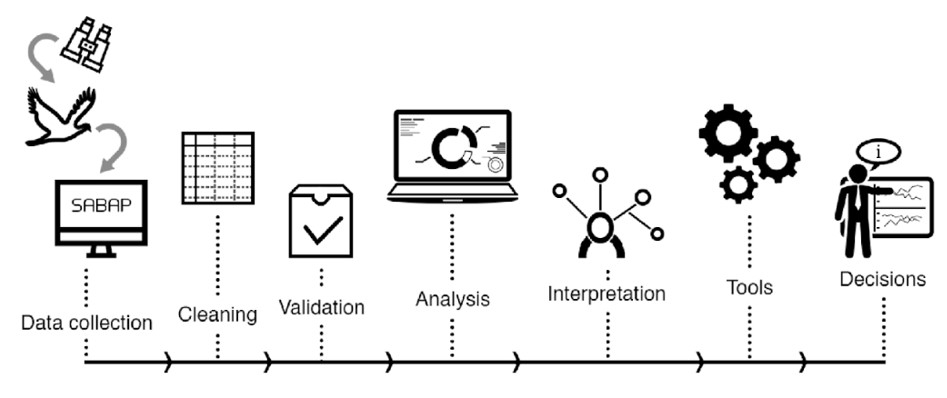
\includegraphics[width=0.9\columnwidth]{figure1_flow.jpg}
  \caption{Basic workflow of the BIRDIE pipeline covering all steps from data collection, to analysis and presentation of digested, decision-ready indicators.}
\end{figure}

\begin{figure}[!h]
\centering
  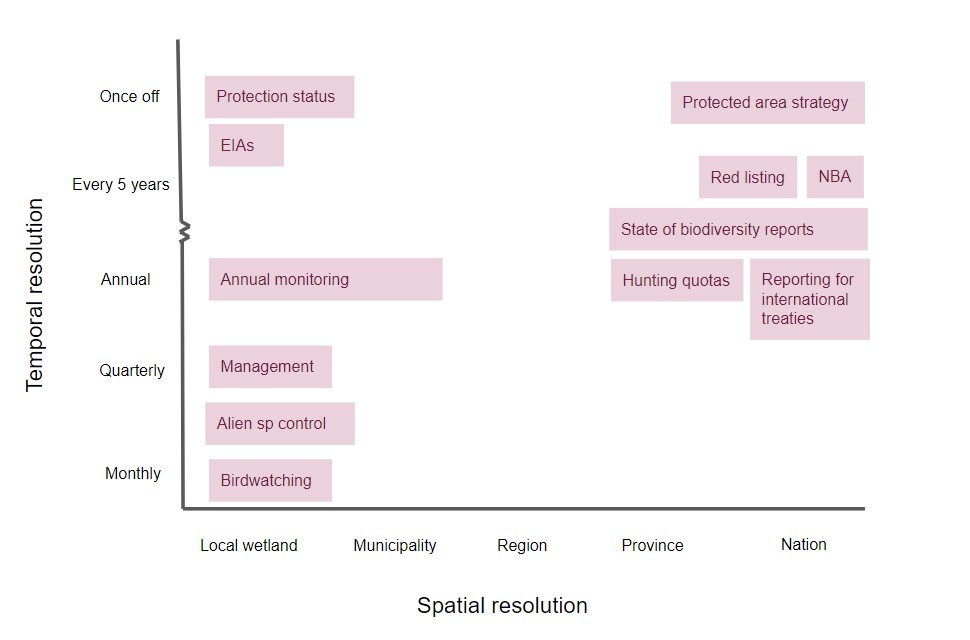
\includegraphics[width=0.9\columnwidth]{figure2_users.jpg}
  \caption{Main users targeted by BIRDIE in relation to their spatial and temporal assessment scales. At present, we focus on computing indicators at an annual temporal resolution or coarser. Finer resolutions are typically based on access to raw data.}
\end{figure}

\begin{figure}[!h]
\centering
  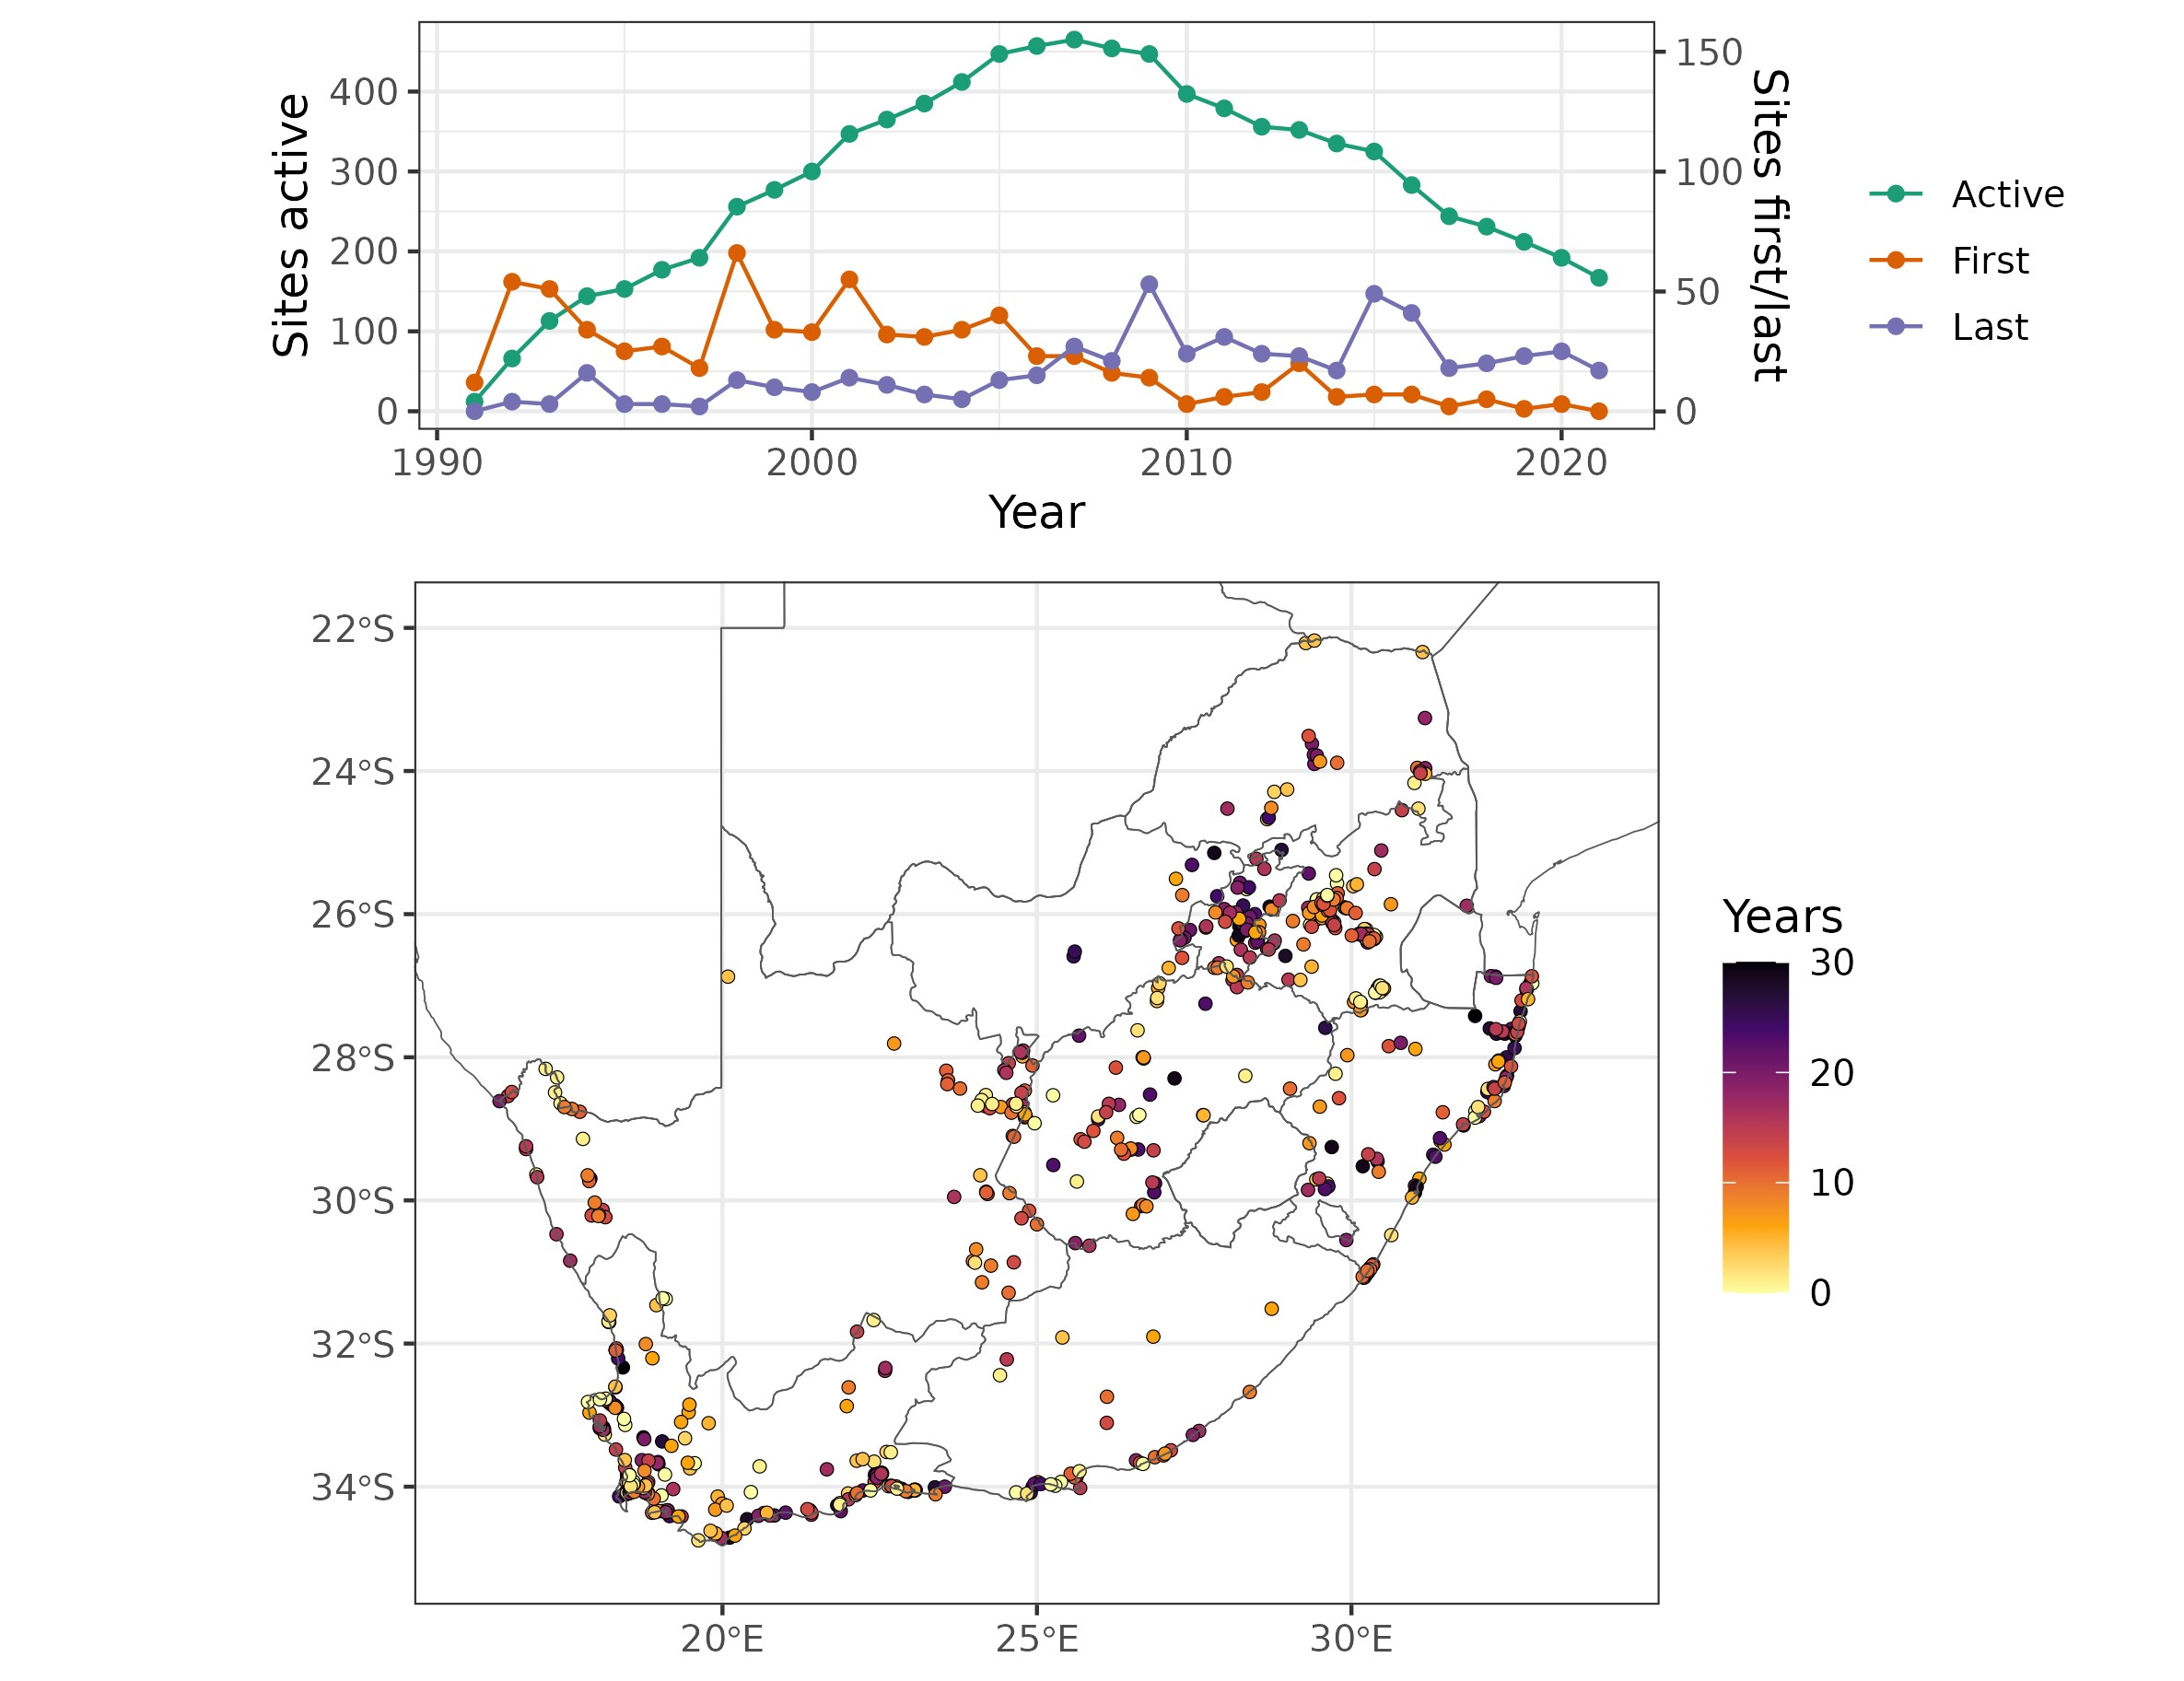
\includegraphics[width=0.9\columnwidth]{figure3_cwac_effort.jpg}
  \caption{The graph shows, the number of CWAC sites active (green), firstly counted (red) and last counted (purple), per year, between 1991 and 2021. Note that some of the sites that were last counted before 2021, might be counted again in the future. In the map, the spatial location of CWAC sites in South Africa. The colour gradient represent the duration of the period the site was counted for.}
\end{figure}

\begin{figure}[!h]
\centering
  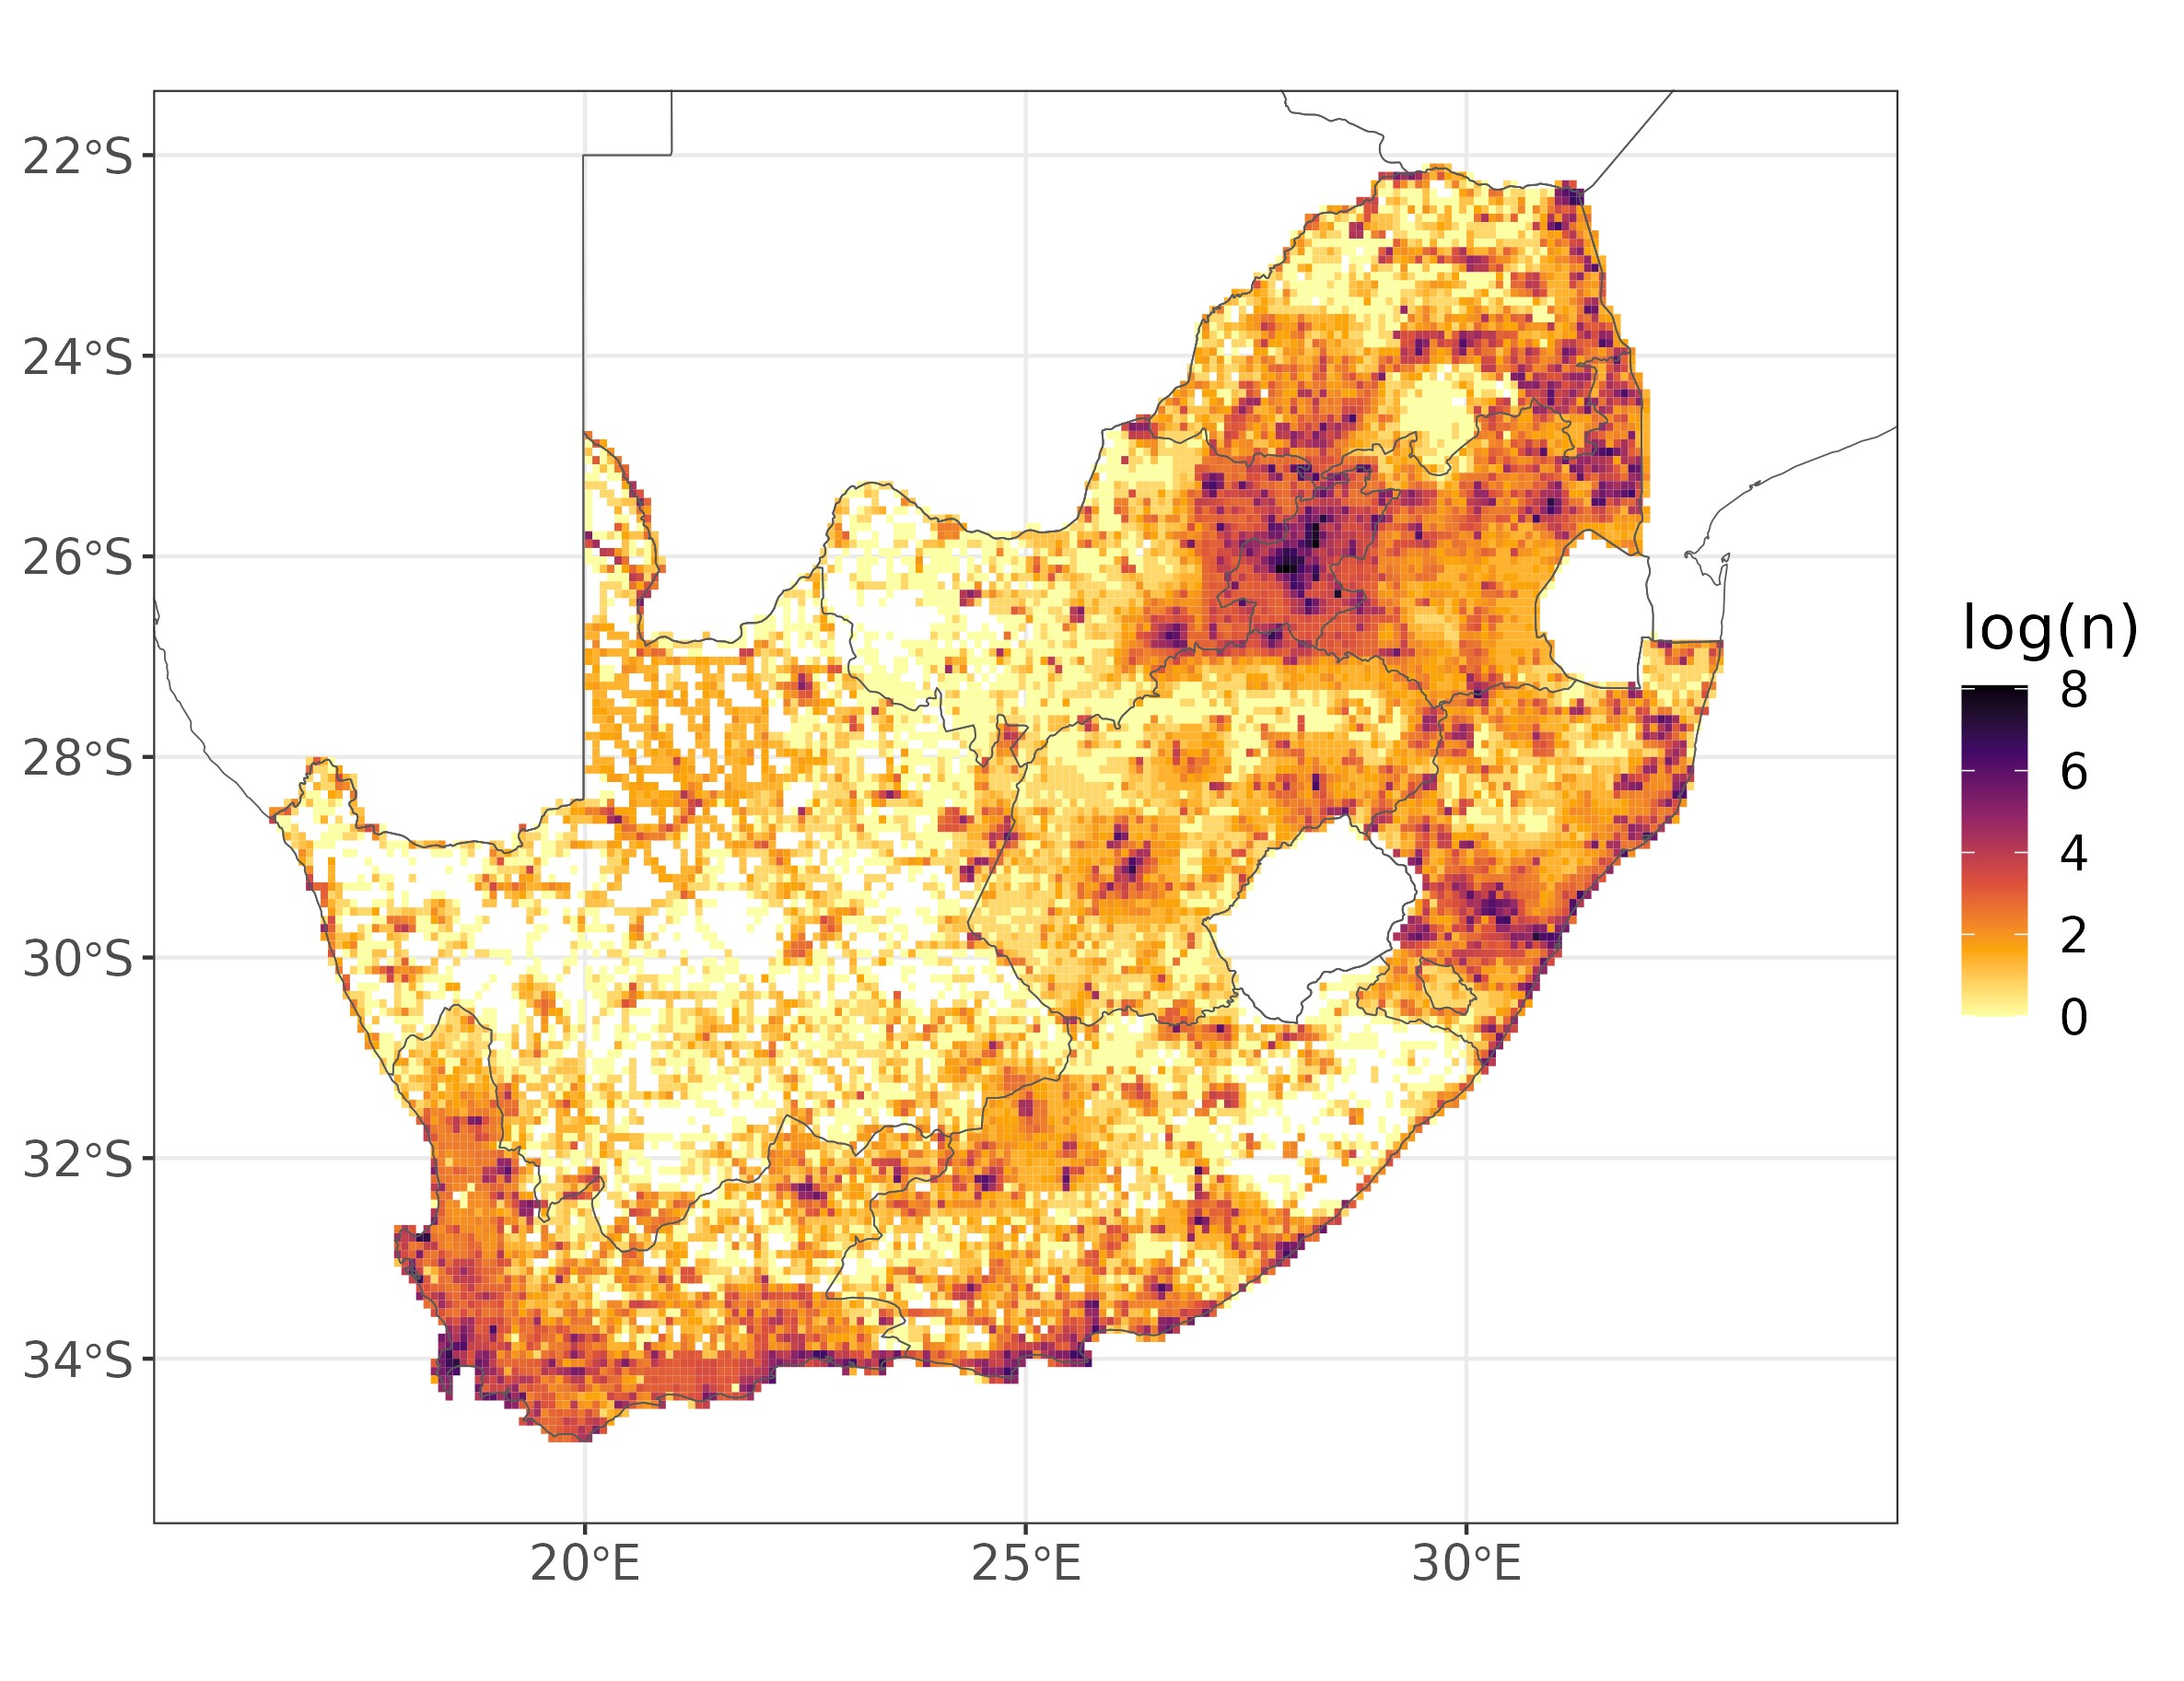
\includegraphics[width=0.9\columnwidth]{figure4_sabap_effort.jpg}
  \caption{Number of SABAP2 cards recorded for the South African pentads between 2008-2021, in logarithmic scale. We can see how areas close to large cities in the Western Cape and Gauteng provinces, accumulate larger efforts. We can also appreciate sampling biased towards roads, particularly in the northwest of the country.}
\end{figure}

\begin{figure}[!h]
\centering
  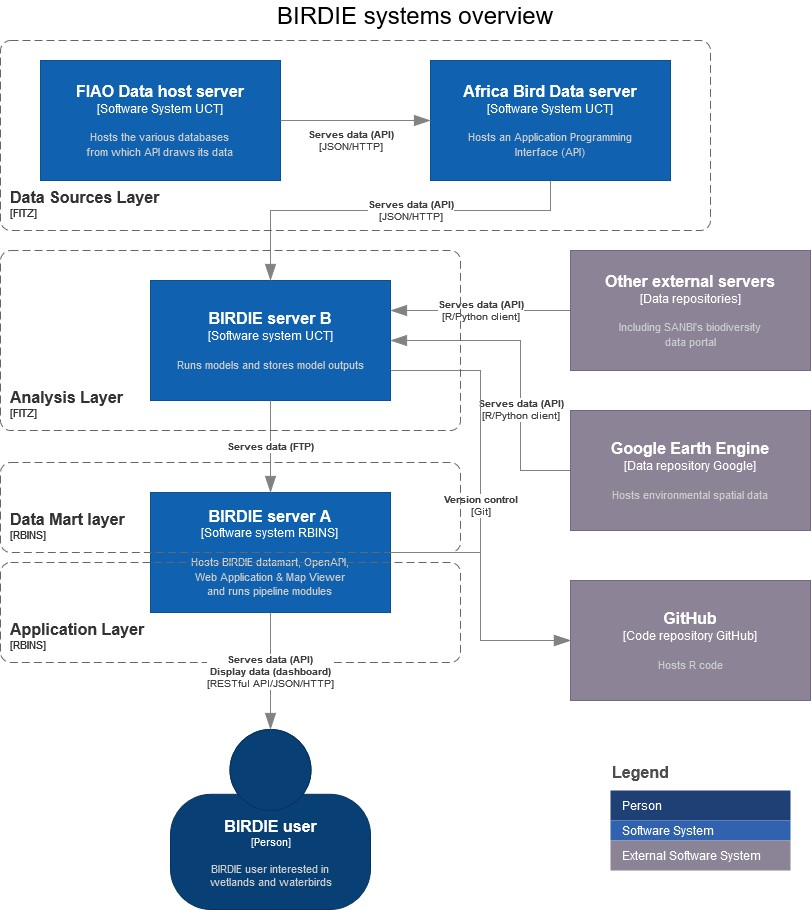
\includegraphics[width=0.9\columnwidth]{figure5_systems.jpg}
  \caption{Overview of BIRDIE’s server architecture. Data flows from CWAC, ABAP and other external servers into BIRDIE server B to be processed and analysed by the R modules, then these outputs move into the data mart in BIRDIE server A, which is the gateway for the dashboard and the final users.}
\end{figure}

\begin{figure}[!h]
\centering
  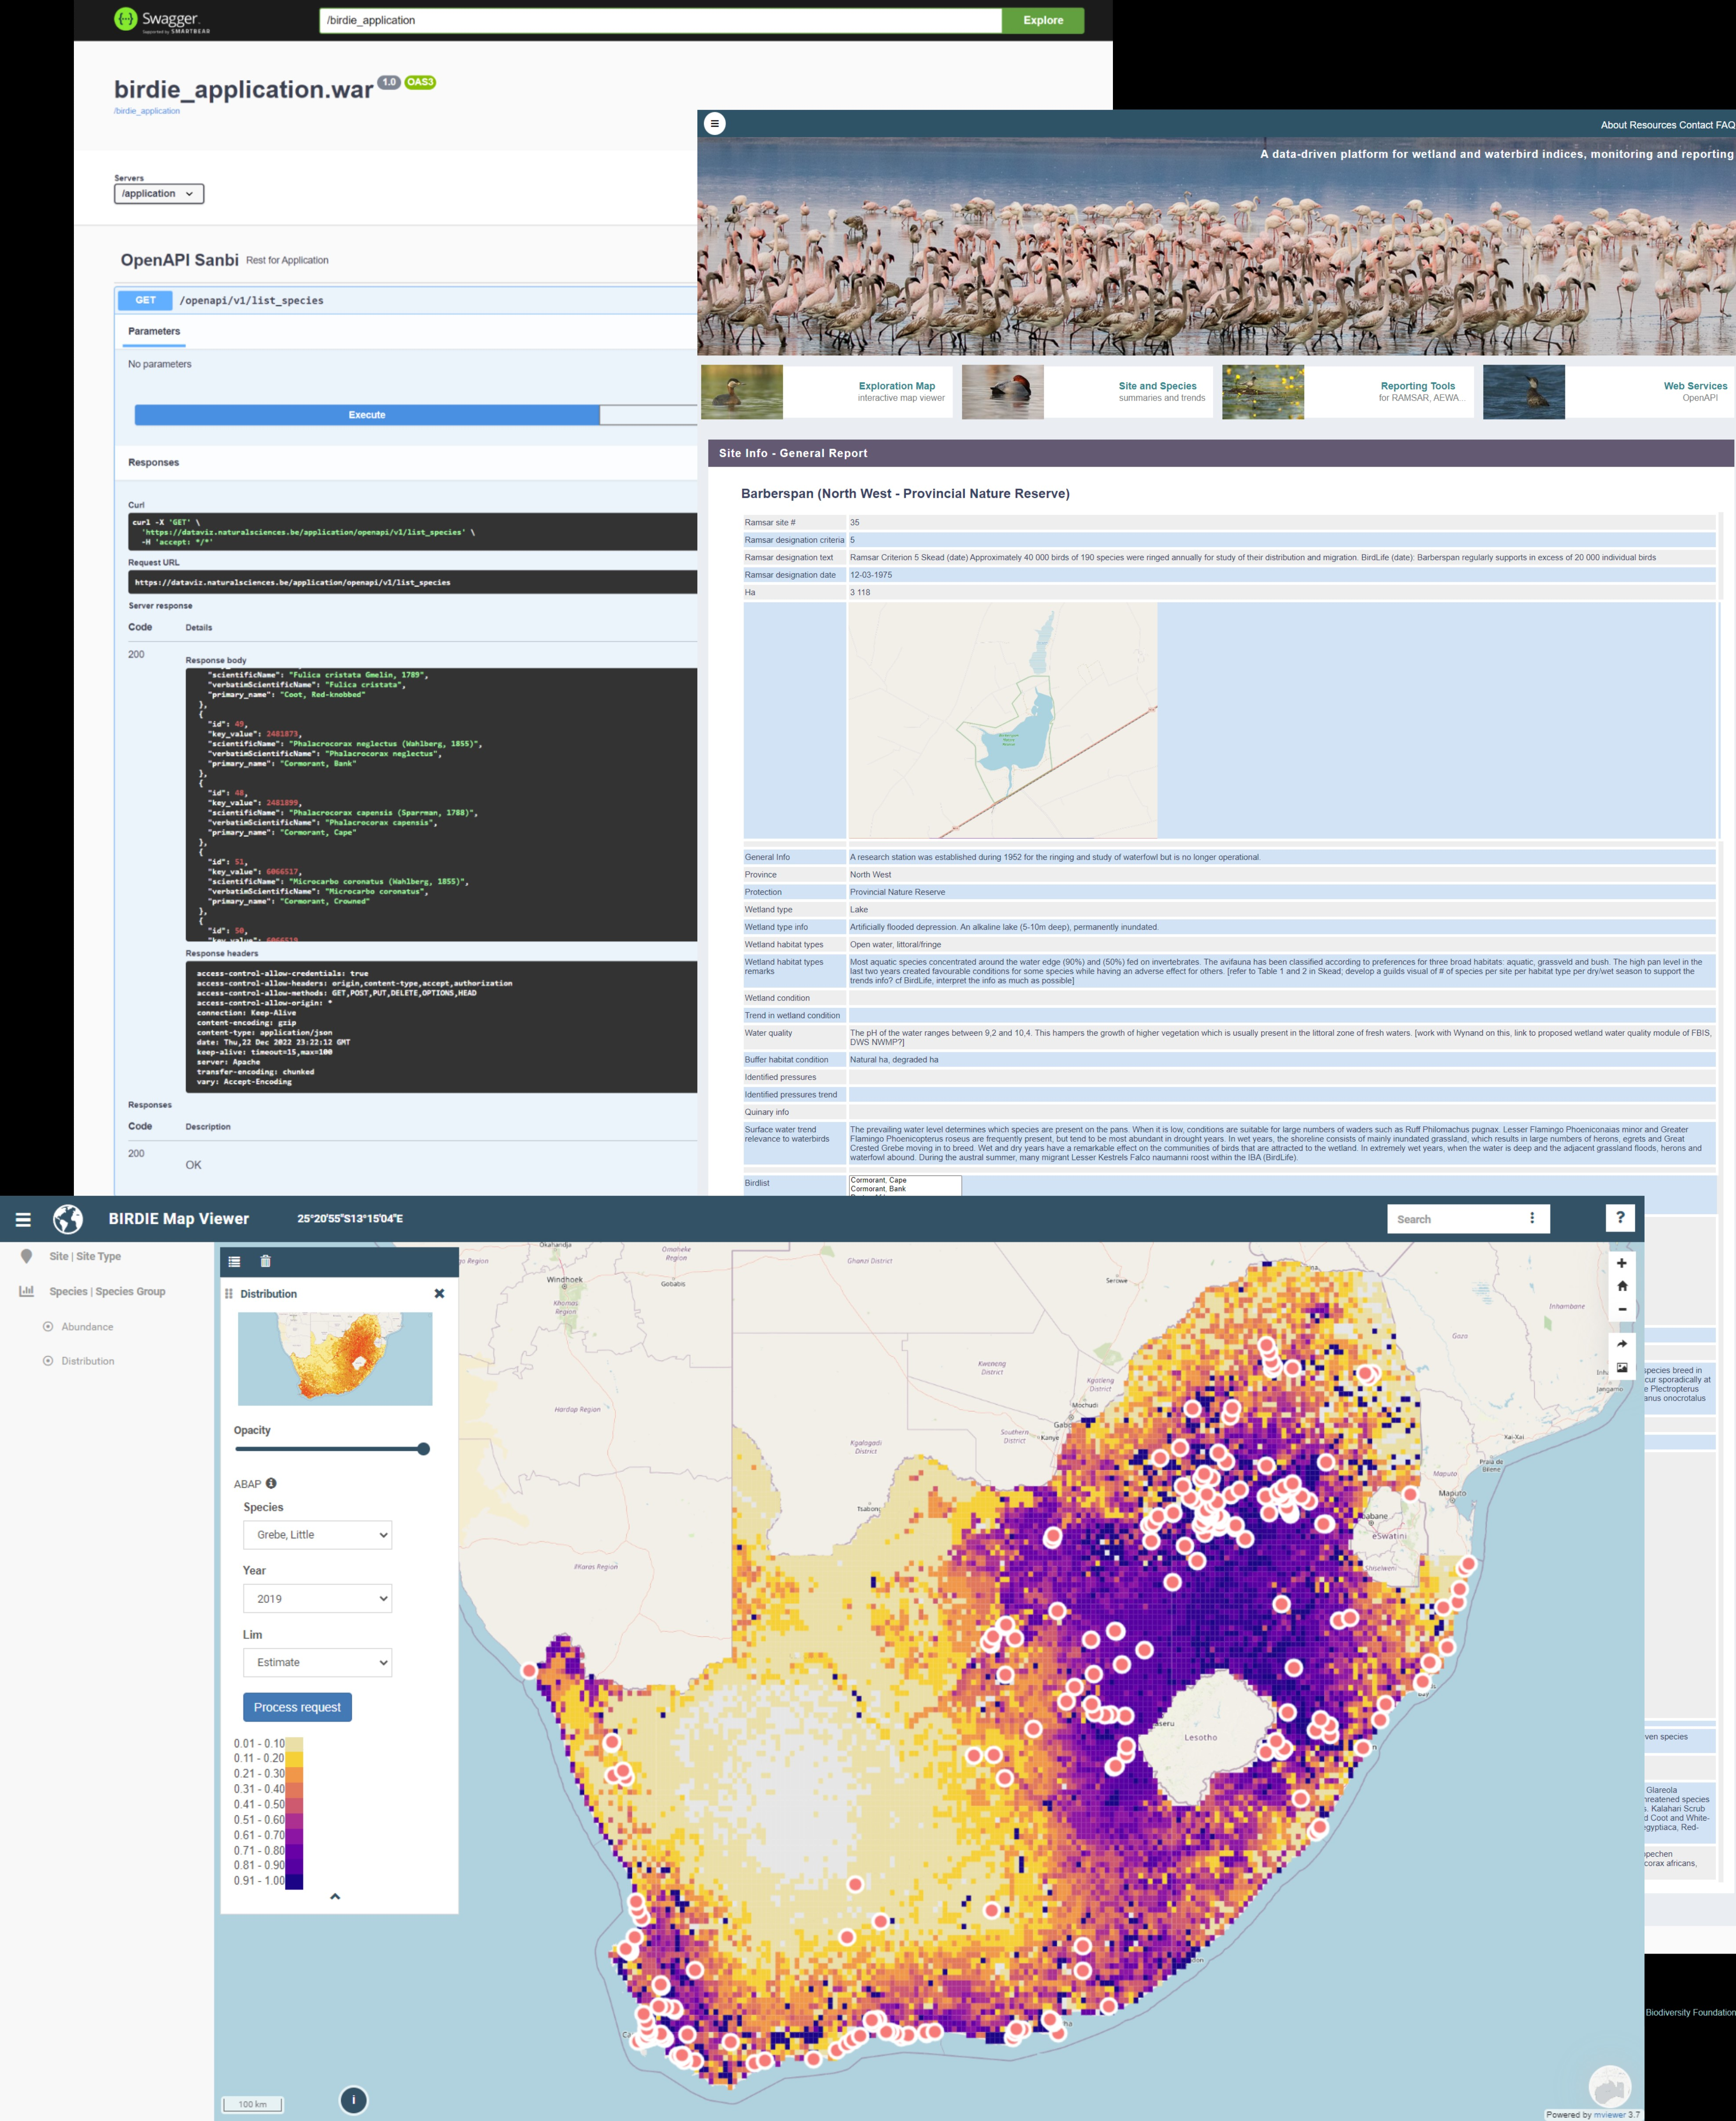
\includegraphics[width=0.9\columnwidth]{figure6_web_app.jpg}
  \caption{Basic elements of the BIRDIE web application: (a) the web services API offers a flexible framework to access the database, facilitating integration with other workflows and platforms, (b) bespoke reports for species, sites and conservation programmes and agreements such as Ramsar or AEWA, and (c) a map viewer that allows flexible exploration of the different BIRDIE indicators.}
\end{figure}

\clearpage

\hypertarget{tables}{%
\section*{Tables}\label{tables}}
\addcontentsline{toc}{section}{Tables}

\begin{table}[h]
\caption{Main indicators produced by the BIRDIE pipeline for waterbird species. For each indicator, we show the inputs, which can be databases (Coordinated Waterbird Counts - CWAC and the African Bird Atlas Project - ABAP), or other indicators; models used to compute the indicator (state-space model -SSM, and occupancy model - Occupancy) or whether it was computed by aggregating other lower-level indicators; the smaller spatial scale of assessment; and the smaller temporal scale of assessment. Annual changes in all of these indicators are also computed, and other indicators will be added over time as needed.}
\begin{tabular}{ |c|c|c|c|c| } 
  \hline
 Indicator & Input & Model & Spatial scale & Temporal scale \\
  \hline
 Abundance & CWAC & SSM & CWAC site & 2 seasons/year \\
Diversity & ABAP & Occupancy & Pentad & Annual \\
Extent of occurrence & Occurrence & Aggregated & National & Annual \\
Area of occupancy & Occurrence & Aggregated & National & Annual \\
Population size & Abundance & Aggregated & National & 2 seasons/year \\
Pop. proportion on site & Abundance & Aggregated & CWAC site/national & 2 seasons/year \\
Waterbird Conservation Value & Abundance & Aggregated & CWAC site/national & 2 seasons/year \\
Number of sites & Abu./occur. & Aggregated & National & Annual \\
 \hline
\end{tabular}
\end{table}


\end{document}
